%****************************************************
%	CHAPTER 2 - Prototype Design
%****************************************************
\chapter{Prototype Design}
\label{ch:proto}
%====================================================
\section{Conventions Used}
\label{sec:proto.conventions}
Here the conventions adopted for the later derived dynamic equations are discussed. Often these aspects relating to conventions are omitted or assumed commonplace. It's important to clearly and unambiguously define a standard set frames so that there can be no uncertainty later in the kinematics.
%====================================================
\subsection{Reference Frames Convention}
\label{subsec:proto.conventions.frames}
%====================================================
\begin{figure}[htbp]
\centering
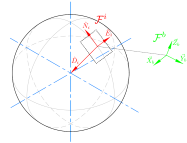
\includegraphics[width=0.6\textwidth]{figs/reference_frame}
\caption{Inertial and Body Reference Frames}
\label{fig:ref_frame}
\end{figure}
Regular aerospace (Euler,\cite{rigidbodylecture}) frames are used for principle inertial and body directions. Shown in Fig: \ref{fig:ref_frame}, the inertial frame,~$\mathcal{F}^i$, is aligned such that the $\vec{X}_i$ axis is in the $\hat{N}$orth direction, $\vec{Y}_i$ is in the $\hat{E}$ast direction and $\vec{Z}_i$ is  in the $\hat{D}$ownward direction\footnote{In orbital sequences this will be toward the Earths' center.}. The body frame, $\mathcal{F}^b$, then has both $\vec{X}_b$ and $\vec{Y}_b$ aligned with two perpendicular arms of the quadrotors' body and finally the $\vec{Z}_b$ axis pointing in the body's normal direction. The relative angular displacement between the two frames is commonly defined by the three angle Euler set, $[\phi ~\theta ~\psi]^T$. An inherent singularity does exists with such attitude representations. Whilst Quaternions are used later in Sec: \ref{subsec:dynamics.rigidbody.quaternion} in lieu of Euler angles, they are easily understood and well suited to illustrate the distinction between rotation and transformation angles which needs to be made.
\par

\subsection{Motor Axis Layout}
\label{subsec:proto.conventions.motoraxis}
%****************************************************

%****************************************************
\section{Design}
\label{sec:proto.design}
%****************************************************
\subsection{Gimbal Articulation}
\label{subsec:proto.design.actuation}
%****************************************************
\subsection{Inertial Matrix Function}
\label{subsec:proto.design.inertia}
%****************************************************
\subsection{Overall Aspects}
\label{subsec:proto.design.aspects}
%****************************************************
\subsubsection{Vibration Damping}
%****************************************************
\subsubsection{Duct}
%****************************************************
\subsubsection{Landing Skids}
%****************************************************
\subsubsection{Motors \& ESCs}
%****************************************************

%****************************************************
\section{System Layout}
\label{sec:proto.layout}
%****************************************************
